%!TEX root=../master.tex

\section{Partner vs Consumer}

\begin{figure}[h]
  \centering
	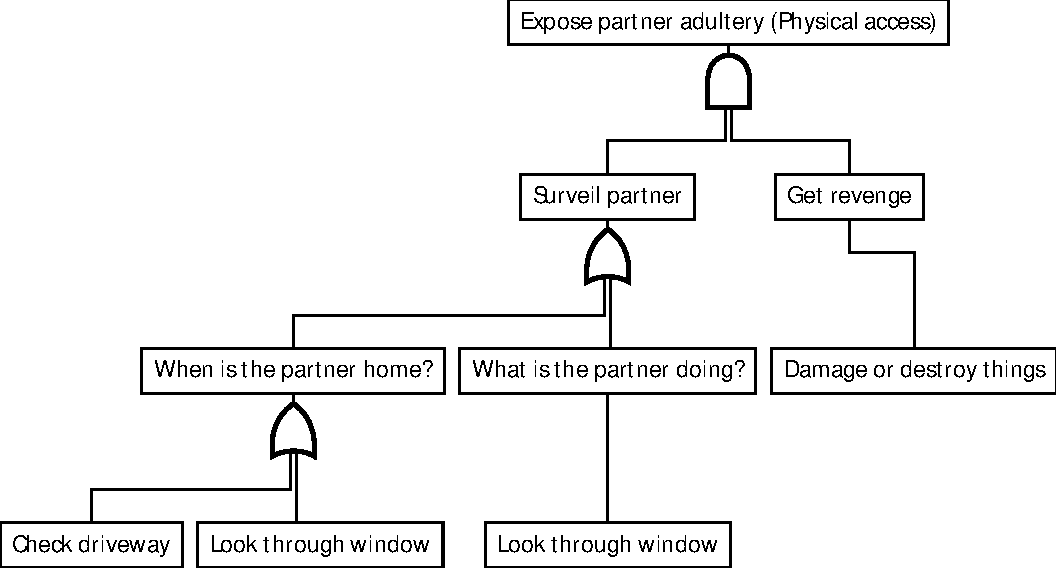
\includegraphics[width=.75\textwidth]{figures/graphviz/partner_vs_consumer_physical.pdf}
	\caption{The Partner vs Consumer -- ``Expose Partner Adultery (Physical access)'' attack tree.}
	\label{fig:attack_trees:partner:cheater_physical}
\end{figure}

\begin{figure}[h]
  \centering
  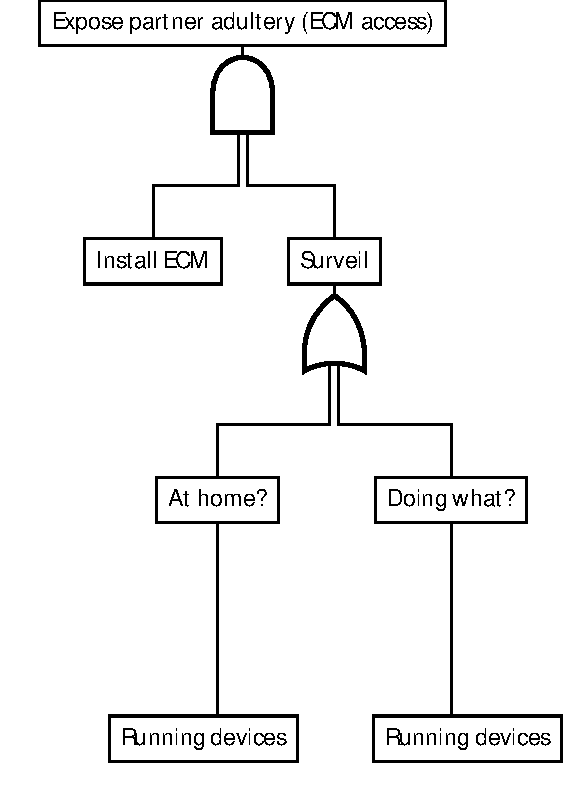
\includegraphics[width=.5\textwidth]{figures/graphviz/partner_vs_consumer_ecm.pdf}
  \caption{The Partner vs Consumer -- ``Expose Partner Adultery (ECM access)'' attack tree.}
  \label{fig:attack_trees:partner:cheater_ecm}
\end{figure}

\begin{figure}[h]
  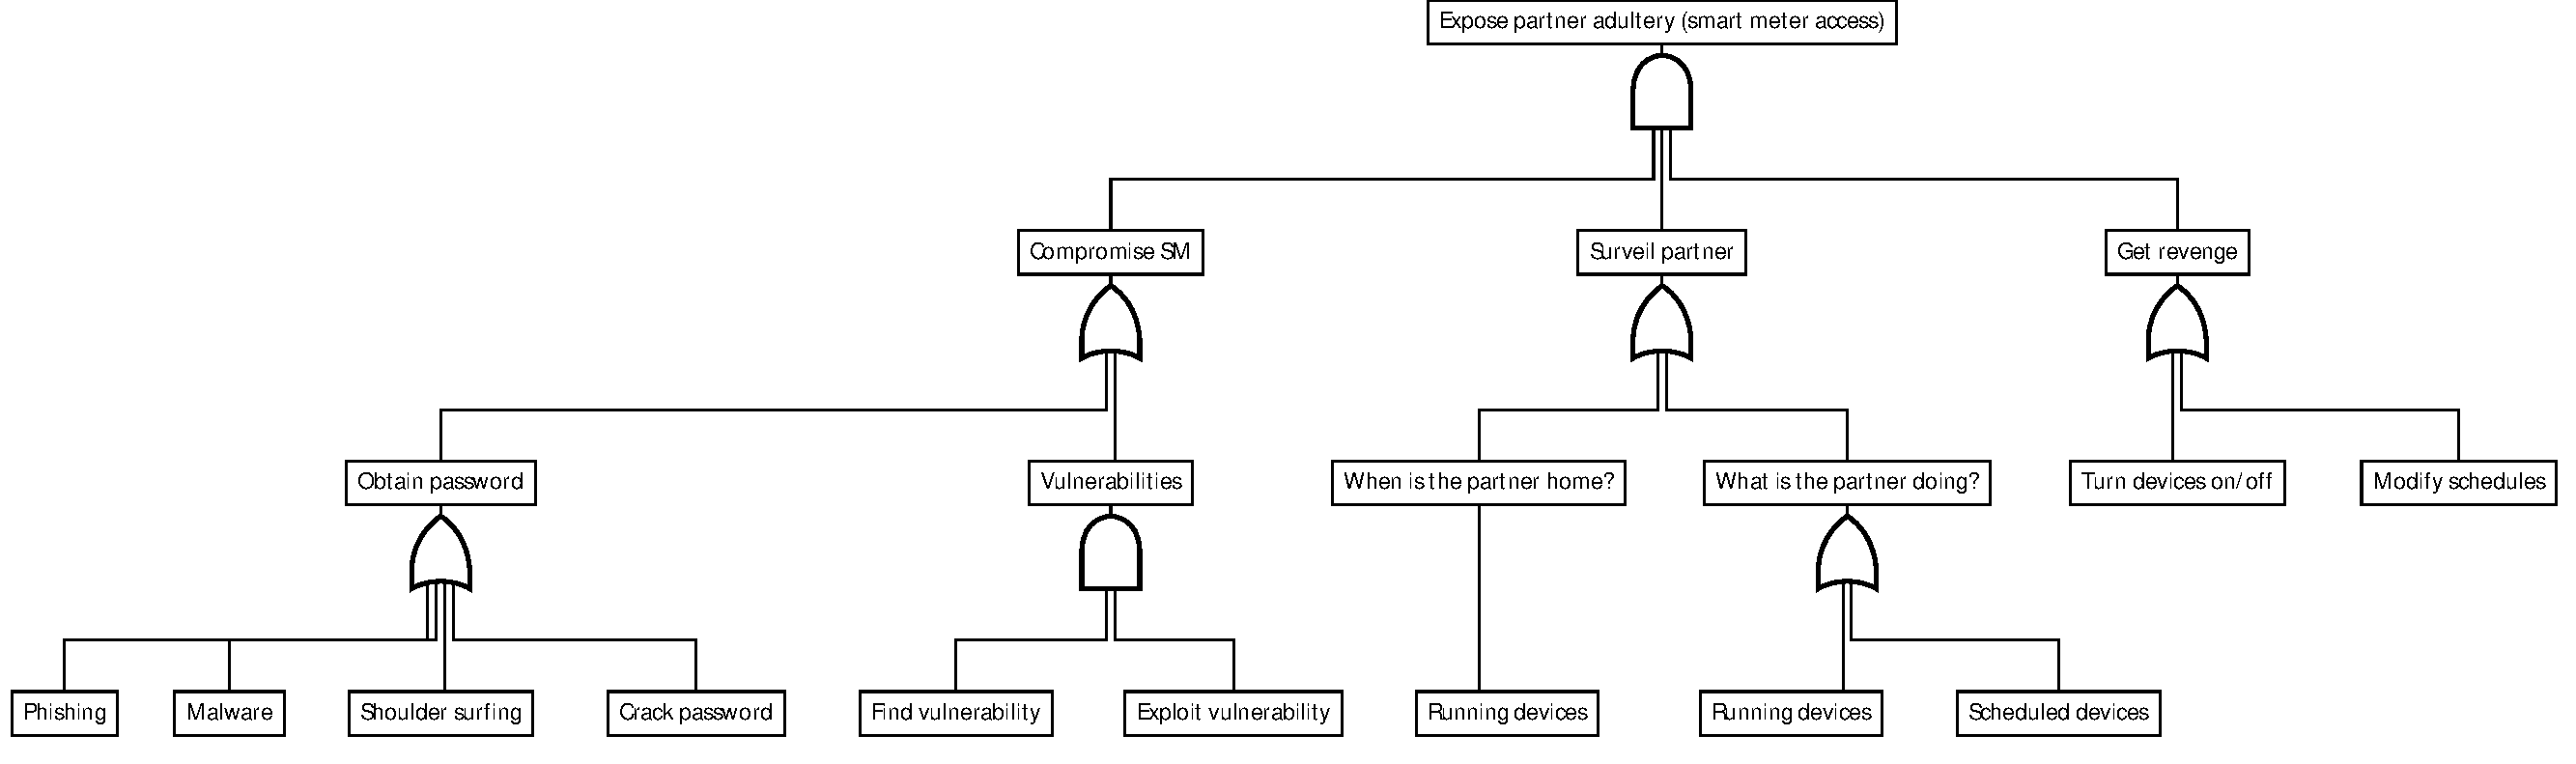
\includegraphics[angle=90,height=\textheight]{figures/graphviz/partner_vs_consumer_sm.pdf}
  \caption{The Partner vs Consumer -- ``Expose Partner Adultery (Smart Meter access)'' attack tree.}
  \label{fig:attack_trees:partner:cheater_sm}
\end{figure}

\begin{figure}[h]
  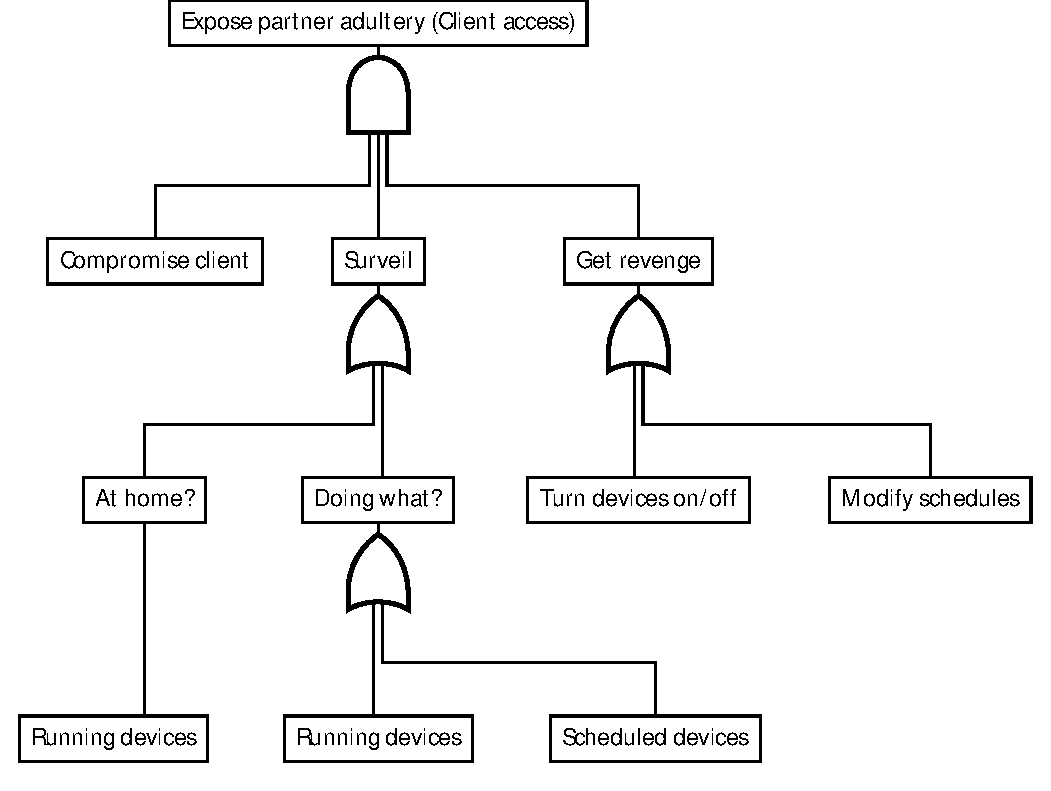
\includegraphics[angle=90,height=\textheight]{figures/graphviz/partner_vs_consumer_client.pdf}
  \caption{The Partner vs Consumer -- ``Expose Partner Adultery (Client access)'' attack tree.}
  \label{fig:attack_trees:partner:cheater_client}
\end{figure}

The partner (or significant other) is an actor with relation to the consumer, but unlike the other actors partners usually can get away with more misdoings inside the consumer's property or house.

\subsection{"Expose Partner Adultery"}

With this attack the partner wishes to monitor the consumer, possibly with following revenge, if monitoring leads to the conclusion that the consumer was cheating on the partner.
What distinguishes the partner's attacks from the burglar or neighbour's is that the partner has increased access to the consumer's property, including the smart meter and related objects.

The attack tree(s) can be seen in \cref{fig:attack_trees:partner:cheater_physical,fig:attack_trees:partner:cheater_ecm,fig:attack_trees:partner:cheater_sm,fig:attack_trees:partner:cheater_client}.
Each tree represents the possible attacks and gains, depending on the kind of access acquired.
There are two or three overall steps to the partner's attack plan: \textit{Gain access, Surveil, Get revenge}, which are repeated in the attack trees.
For any other attack than physical, some kind of access to gain information is required.

\subsubsection{Access}
First of all the partner needs to gain access which can give the partner valuable insight into the doings of the consumer.
In relation to power consumption, the partner has three ways of accessing the consumer's data, which could give the partner the details the partner need to determine whether the consumer is home or not.

The partner could install an external consumption monitor\footnote{E.g. a TED (The Energy Detective) used in \cref {smart_meter_privacy}.} on the power grid in the house, giving the partner direct power consumption data.
Assuming that the consumer is using a client, in the form of a tablet or other smart device, to monitor the power consumption, the partner could gain access to one of these devices.
Finally, the partner could tamper directly with the smart meter, similar to the neighbour's or burglar's smart meter attacks.

\subsubsection{Surveillance}
The main goal of this attack is to surveil and through this surveillance expose the consumer's misdeeds.
The nodes regarding devices are dependant on gained access through the \textit{Gain access} sub-tree as is represented with individual attack trees based on acquired access.

The partner first option is physical presence, such as looking through a window.
However, assuming that the partner was able to somehow get hold of the consumer's power consumption data, the partner now has options to expose the consumer from a distance.

First of all, the partner could determine whether the consumer is home, and shouldn't be, or that the consumer isn't home, but should be.
This can be done by looking at which devices are scheduled for tasks or from looking at the device power signatures.
The same method can be used to determine what the consumer is doing if the consumer is home, such as brewing more coffee than usual or taking unusually long showers.
See \cref{smart_meter_privacy} to see how to obtain this information from consumption data.

\subsubsection{Revenge}
The final step of the attack plan is an optional cold dish of revenge.

The partner could of course destroy stuff by applying physical manipulation in one way or another.
However, if the partner wanted to get creative, the partner could use the partner previously gained access to the smart meter to manipulate the consumer psychologically.
The partner could turn on/shut off the consumer's appliances at inconvenient times.
If the partner wanted to get even more creative, the partner could modify the appliances' schedules such as turning everything on at late night with low intervals.
